\chapter{JPaxos user guide}

\section{Overview}
\label{overview:overview}\label{overview::doc}\label{overview:jpaxos-user-guide}
JPaxos is a Java library and runtime system for efficient state machine
replication. \linebreak With JPaxos it is very easy to make a user-provided
service tolerant to machine crashes. Our system supports the \emph{crash-recovery}
model of failure and tolerates message loss and communication delays.
\begin{description}
\index{State machine replication}\item[{\href{http://en.wikipedia.org/wiki/State\_machine\_replication}{State machine replication}}] \leavevmode\phantomsection\label{overview:term-state-machine-replication}
is a general method for implementing a fault-tolerant service by
replicating it on separate machines and coordinating client interactions
with these replicas (or copies). The physical isolation of machines in
a distributed system ensures that failures of server replicas are
independent, as required. \linebreak As long as there are enough of non-faulty
replicas, the service is guaranteed to be provided.

\end{description}

JPaxos makes the following assumptions about the replicated service:
\begin{itemize}
\item {} 
deterministic behaviour, i.e. multiple copies of the service begun in
the start state, receiving the same inputs in the same order will
arrive at the same state having generated the same outputs

\item {} 
non-Byzantine failures, i.e. a service machine can only crash

\item {} 
crash-recovery supported, i.e. after crash, the service can be restarted
with the same IP address.

\end{itemize}


\subsection*{A.1.1\quad Two execution modes}
\label{overview:two-execution-modes}
JPaxos can be run in one of the following two modes of operation
(the mode is set up from the configuration file at system start up
and cannot be changed at runtime):

Basic mode
\begin{itemize}
\item {} 
to be able to tolerate $f$ faulty replicas, the system must consists
of at least $2f + 1$ replicas (i.e. $n \ge 2f + 1$)

\item {} 
after replica crash, it recovers its state from other replicas

\end{itemize}

Extended mode
\begin{itemize}
\item {} 
no limit on the number of faulty processes (i.e. $f = n$)

\item {} 
after replica crash, it recovers its state from non-volatile memory

\item {} 
around 200 times slower than the basic mode

\end{itemize}


\subsection*{A.1.2\quad Simple API}
\label{overview:simple-api}
For the end user JPaxos provides:
\begin{enumerate}
\item {} 
\code{Service} interface -- it specifies a few methods for interfacing
the user-defined servi\-ce code with JPaxos; our library provides
abstract classes implementing \code{Ser\-vice} interface, making it easier to
to create a new service (state machine);\linebreak
see {\hyperref[api:jpaxos-service]{\emph{Service interface}}} for details

\item {} 
\code{Replica} class -- that should be instantiated and started
(see {\hyperref[api:jpaxos-replica]{\emph{Replica}}} for details)

\item {} 
\code{Client} class -- the part that may send request to be executed
(see {\hyperref[api:jpaxos-client]{\emph{Client}}} for details)

\end{enumerate}

The \code{Service} and \code{Replica} are bound to each other, while
\code{Client} can be located anywhere.

JPaxos guarantees that in crash-recovery model, with static groups,
lossy network with any delays:
\begin{itemize}
\item {} 
if the client sends a request, it will eventually get the answer

\item {} 
every replica will execute the request exactly once

\item {} 
any two replicas will execute the requests in the same order

\end{itemize}


\subsection*{A.1.3\quad Distributed implementation}
\label{overview:distributed-implementation}
JPaxos is a fully distributed implementation, which means that there
is no predefined central coordinator that might be a bottle-neck or a single
point of failure in the system.

For this, JPaxos implements
the \href{http://en.wikipedia.org/wiki/Paxos\_algorithm}{Paxos}
distributed algorithm with various optimizations, in order to efficiently
deliver client requests to all service replicas despite any failures.
Replicas receive all requests globally ordered, thanks to
the total-order (or atomic) broadcast protocol implemented on top
of Paxos.

Figure below shows processing of a single request message submitted
by the Client to the replicated state machine:
\begin{quote}
\begin{figure}[htbp]
\centering

\scalebox{0.750000}{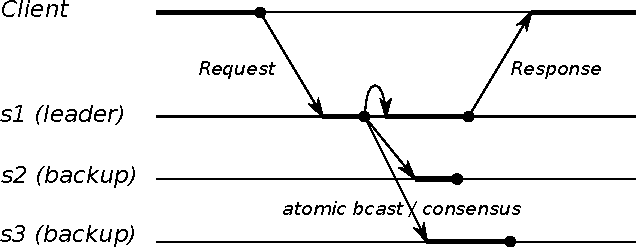
\includegraphics{user_guide/state_machine.pdf}}
\end{figure}
\end{quote}

where \emph{Client} is an instance of the \code{Client} class, while \emph{s1}, \emph{s2},
and \emph{s3} are instances of the \code{Replica} class.

If a request is delayed or lost due to the network or replica failure,
after a timeout, it will be reissued by the \emph{Client}, as illustrated in
Figure below:
\begin{quote}
\begin{figure}[htbp]
\centering

\scalebox{0.750000}{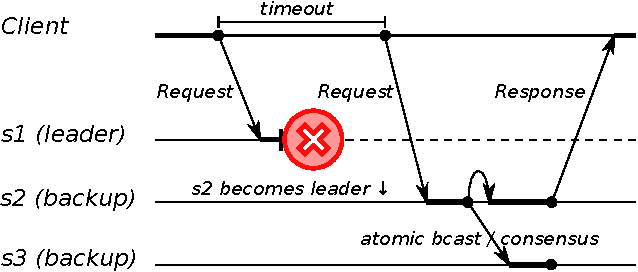
\includegraphics{user_guide/state_machine_crash.pdf}}
\end{figure}
\end{quote}


\section{Deployment and configuration}
\label{config:deployment-and-configuration}\label{config::doc}
This section presents quick overview on what is necessary to compile the
library and how to configure the system and start the example which is included
in the distribution.


\subsection{Deployment requirements}
\label{config:deployment-requirements}
JPaxos requires the following components to be installed on the target system:
\begin{itemize}
\item {} 
\href{http://www.java.com/}{Java JRE 1.5} or later

\end{itemize}

Additionally, the following are optional but helpful tools in compilation and
packaging:
\begin{itemize}
\item {} 
\href{http://ant.apache.org/}{Apache Ant} -- used to run all build scripts (distributed under the Apache
License 2.0)

\end{itemize}


\subsection{Configuration file}
\label{config:configuration-file}
The format of configuration file used by \code{Configuration} class is the same as
default Java Properties file. As mentioned earlier, this file contains
nodes configuration and replica related options.


\paragraphNewline{Node configuration}
\label{config:node-configuration}
A node is configured with a single line containing \code{hostname}, \code{replica
port} and \code{cli\-ent port}, separated with commas:

\begin{Verbatim}[commandchars=@\[\]]
process.@textless[]id@textgreater[] = @textless[]hostname@textgreater[]:@textless[]replica@_port@textgreater[]:@textless[]client@_port@textgreater[]

process.0 = localhost:2000:3000
process.1 = localhost:2001:3001
process.2 = localhost:2002:3002
\end{Verbatim}

Above configuration creates three replicas with ids: 0, 1, 2. Replica with id 0,
is running on localhost and is using port 2000 to communicate with other replicas
and is using port 3000 to accept connections from clients.


\paragraphNewline{Crash model selection}
\label{config:crash-model-selection}
One should select the crash model of the system. If the crash model uses the
non-volatile memory (i.e. hard drive), the location of the logs may be
specified as well.

Currently supported crash models include:

\begin{tabular}{|L|L|L|L|}
\hline
\textbf{
Type
} & \textbf{
Name
} & \textbf{
Needs stable storage
} & \textbf{
Fault tolerance
}\\
\hline

CrashStop
 & 
CrashStop
 & 
No
 & 
minority
\\

CrashRecovery
 & 
FullStableStorage
 & 
Yes, heavy usage
 & 
catastrophic
\\

CrashRecovery
 & 
ViewSS
 & 
Yes, periodically
 & 
minority
\\

CrashRecovery
 & 
EpochSS
 & 
Yes, one write by start
 & 
minority
\\
\hline
\end{tabular}

\begin{description}
\item[{Crash model types:}] \leavevmode\begin{itemize}
\item {} 
CrashStop -- once the replica crashed, it cannot recover

\item {} 
CrashRecovery -- the replica may crash and subsequently recover

\end{itemize}

\end{description}

Fault tolerance ranks:
\begin{itemize}
\item {} 
minority -- the minority of replicas may crash; $f = \left\lfloor (n-1)/2 \right\rfloor$

\item {} 
catastrophic -- all replicas may crash; $f=n$

\end{itemize}

To select a crash model, one must add to the configuration file a line
\\\code{CrashModel = {[}crash model name{]}}\\ If no crash model is provided, the
\code{FullStableStorage} is assumed.

For choosing a log path one needs to add another line with syntax\\ \code{LogPath =
{[}path{]}}\\ The logs will be actually stored in subdirectory named after replica
id in the given location. The default value for log path is \code{jpaxosLogs}.

An example configuration:

\begin{Verbatim}[commandchars=@\[\]]
CrashModel = ViewSS
LogPath = /mnt/shared/jpaxos/logs
\end{Verbatim}


\paragraphNewline{Replica options}
\label{config:replica-options}
Configuration file also allows to set additional options for replicas.
Understanding how each option described below can affect JPaxos is important to
achieve high performance.


\paragraphNewline{Window size}
\label{config:window-size}
The window size determines the maximum number of concurrently proposed
instances. The meaning of this option is very similar to window size in TCP
protocol.

To illustrate it, assume that window size is set to 10. It allows to run
instances with IDs from 1 to 10 concurrently and to decide instances 2 -- 10
before instance 1. JPaxos cannot execute any instance until all previous
instances are executed so because instance 1 is not decided / executed, no
instance can be executed on state machine. When instances 1 will be
decided and executed all consecutive instances will also be executed.

The example above shows that by increasing the value of window size we can
decrease the response time -- a lot of instances will be decided, but none can
be executed. Because of that it is recommended to set this option to lower
value and BatchSize to higher value so that decided instances can be executed
faster.

The default value of this option is 2 and can be set using:
\begin{Verbatim}
WindowSize = 4
\end{Verbatim}

\paragraphNewline{Batch size}
\label{config:batch-size}
JPaxos will try to batch requests into a single proposal to improve the
performance. This option controls the maximum size (in bytes) of requests
grouped into one consensus instance.

For example, if maximum batch size is set to 1000 and JPaxos received requests
of size 100, 300, 400, 300 bytes, then first three requests will be batched
into one consensus instance of size 100 + 300 + 400 = 800 (the size of all four
requests is 1100 what is greater than maximum allowed batch size).

The default value of this options is 65507 bytes and can be changed by adding:
\begin{Verbatim}
BatchSize = 65507
\end{Verbatim}


\paragraphNewline{Maximum batch delay}
\label{config:maximum-batch-delay}
This option determines how long JPaxos will wait for new requests to be packed
into single instance.

The default value of this option is 10 ms and can be change using:
\begin{Verbatim}
MaxBatchDelay = 20
\end{Verbatim}


\paragraphNewline{Network protocol}
\label{config:network-protocol}
It is also possible to choose protocol used to communicate between replicas.
One may choose:
\begin{itemize}
\item {} 
TCP (default)

\item {} 
UDP

\item {} 
Generic -- Uses UDP for small messages and TCP for larger messages

\end{itemize}

It is important to note that UDP protocol has message size restriction -
messages must be smaller than the maximum allowed size of UDP packet (64KB or
less, depending on the network). User must be careful with the size of client
requests and of BatchSize so that this limit is not violated. Because of this
limitations, user should choose TCP or Generic option.

If one chooses Generic, it is also recommended to set what is a `small' and
what is a~`big' message, by setting maximum allowed UDP packet size:

\begin{Verbatim}[commandchars=\\\{\}]
\PYG{n}{Network} \PYG{o}{=} \PYG{n}{Generic}
\PYG{n}{MaxUDPPacketSize} \PYG{o}{=} \PYG{l+m+mi}{1000}
\end{Verbatim}

In example above, all messages smaller than 1000 bytes will be sent using UDP
and all others using TCP protocol.

\paragraphNewline{Example file}
\label{config:example-file}

Below is an example configuration file:

\begin{Verbatim}[commandchars=@\[\]]
@# Nodes configuration
process.0 = 192.168.1.5:2000:3000
process.1 = 192.168.1.6:2001:3001
process.2 = 192.168.1.7:2002:3002

@# Crash model configuration
CrashModel = EpochSS
LogPath = jpaxos/stableStorage

@# Batching configuration
WindowSize = 2
BatchSize = 65507
MaxBatchDelay = 10

@# Network configuration
Network = TCP
\end{Verbatim}


\subsection{Configuration classes}
\label{config:configuration-classes}
The user of JPaxos has to configure the system by creating instance of
\code{Configuration} class. Instance of this class is required to create the
\code{Replica} and \code{Client} (see {\hyperref[api:jpaxos-api]{\emph{Application programming interface}}} chapter).

The \code{Configuration} class either loads the setting from certain file, or the
settings may be provided by instantiating.

\code{Configuration} contains nodes configuration (information about replicas -- ids,
hostnames and ports), and replica related options (batching size, window size,
etc.). \code{Client} is using only nodes configuration (hostnames and ports) and
ignores replica related options, while \code{Replica} is using all options from
\code{Configuration}.

The user is responsible for providing correct configuration to replicas and
clients. The configuration must be the same in every replica and client or else
the system may fail.


\paragraphNewline{\texttt{Configuration} class}
\label{config:jpaxos-configclass}\label{config:configuration-class}
The \code{Configuration} has three constructors available:
\begin{itemize}
\item {} 
\code{Configuration ()}
Default constructor, loads configuration from \code{paxos.pro\-per\-ties} file
located in current working directory. The structure of configuration file is
described in ``Configuration file format'' section.

\item {} 
\code{Configuration (String fileName)}
Loads configuration from file specified as constructor argument. The format
of the file is described in ``Configuration file format'' section.

\item {} 
\code{Configuration (List\textless{}PID\textgreater{} processess)}
Loads configuration using only no\-des configuration. The \code{PID} structure is
described below. Replica related options are set to default.

\end{itemize}


\paragraphNewline{\texttt{PID} class}
\label{config:pid-class}
Stores node configuration data (information about one replica):
\begin{itemize}
\item {} 
\code{id}
The id of replica. Ids start from 0.

\item {} 
\code{hostname}
The replica ip address (e.g. ``127.0.0.1'') or host name (e.g. ``localhost'').
The replicas (and clients) will use this address to establish connection with
this replica.

\item {} 
\code{replicaPort}
The port used by replicas to establish connection with this replica.

\item {} 
\code{clientPort}
The port used by clients to establish connection with this replica.

\end{itemize}


\section{Application programming interface}
\label{api:application-programming-interface}\label{api:jpaxos-api}\label{api:code-generation-library}\label{api::doc}

%\subsection{Introduction}
%\label{api:introduction}
A non-replicated service looks like this:
\begin{figure}[H]
\centering
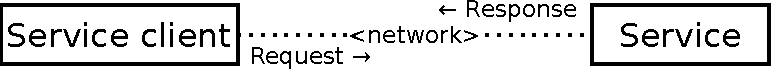
\includegraphics[width=20em]{user_guide/api_sm.pdf}
\end{figure}

\noindent\ignorespaces Our library replaces the \code{\textless{}network\textgreater{}} part. It looks like:
\begin{figure}[H]
\centering
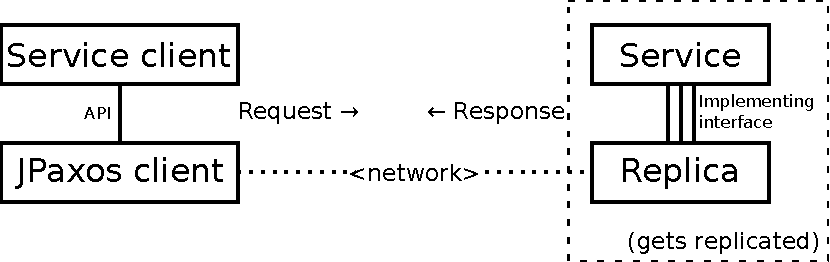
\includegraphics[width=20em]{user_guide/api_jpaxos.pdf}
\end{figure}

In order to make the replication and recovery possible, we require a few additional methods from the Service.

JPaxos provides implementation of its Client and the Replica. The programmer must implement the Service and make use of the Client class.

\code{Client} sends requests to replicas and waits for reply. It provides only method for connecting and executing requests.

\code{Replica} uses Paxos algorithm to order client requests in all replicas; after deciding requests, executes them on service in proper order. All methods from \code{Service} class are called from one \code{Replica} thread, that means no two will be called concurrently on the service.

\code{Service} executes all requests from clients deterministically. The service must also implement a few additional methods to save and restore its state, which will explained in detail below.

Data exchanged by client and service are in form of byte arrays -- \code{byte{[}{]}}. This gives biggest flexibility to the programmer -- any data can be put there. One may use byte arrays in the service, as well as serialise/deserialise the \code{byte{[}{]}} to certain objects.


\subsection{Service}
\label{api:service}
JPaxos provides several base classes and one interface to create a new Service.

The \code{Service} interface, base for all services, describes methods that JPaxos requires from the service to be implemented. \code{Replica} calls all the API methods on the \code{Service} object. To launch the service, one needs to start the governing \code{Replica}.

\clearpage

The inheritance hierarchy is as follows:

\begin{Verbatim}[commandchars=@\[\]]
interface Service
  abstract class AbstractService
    abstract class SimpleService
      abstract class SerializableService
\end{Verbatim}

Using the \code{Service} interface is discouraged in favour of \code{AbstractService}, as the latter implements methods common to all services.

\code{AbstractService} provides widest range of functionality. \code{SimpleService} is the \code{AbstractSer\-vice} narrowed to the absolute minimum for the system to work. \code{Seria\-li\-za\-ble\-Service} differs from \code{SimpleService} only with data type -- all client requests and service responses are serialised using Java serialisation.


\paragraphNewline{\texttt{SerializableService} class}
\label{api:serializableservice-class}
This is the simplest class of all available.

This class has minimal number of methods. One requires from the \code{Serializable\-Service} to be able to execute client requests, be able to create a snapshot and roll back to state from a snapshot.

\code{SerializableService} uses Java serialization for creating byte arrays from Object, therefore snapshot, request and reply classes must be serialisable.

Method summary:
\begin{itemize}
\item {} 
\code{abstract Object execute (Object value)}
\begin{quote}

Executes a command from client on this state machine. The return value is sent back to the client.
\end{quote}

\item {} 
\code{abstract Object makeSnapshot ()}
\begin{quote}

Makes snapshot of current Service state. The same data created in this method, will be used to update state from snapshot using \code{updateTo\-Snap\-shot(Object)} method.
\end{quote}

\item {} 
\code{abstract void updateToSnapshot (Object snapshot)}
\begin{quote}

Updates the current state of Service to state from snapshot. This me\-thod will be called after recovery to restore previous state, or if we received newer snapshot from other replica (using catch-up).
\end{quote}

\end{itemize}


\paragraphNewline{\texttt{SimplifiedService} class}
\label{api:simplifiedservice-class}
This class also has minimal number of methods.

Only difference between \code{Simplified\-Ser\-vice} and \code{SerializableService} is the type of passing the data -- the \code{SimplifiedService} uses byte arrays for that.

Method summary:
\begin{itemize}
\item {} 
\code{abstract byte{[}{]} execute (byte{[}{]} value)}

\item {} 
\code{abstract byte{[}{]} makeSnapshot ()}

\item {} 
\code{abstract void updateToSnapshot (byte{[}{]} snapshot)}

\end{itemize}


\paragraphNewline{\texttt{AbstractService} class}
\label{api:abstractservice-class}
This class supports three additional functionalities in comparison to \code{Simplified\-Ser\-vice} and \code{SerializableService}:
\begin{itemize}
\item {} 
service may choose when the snapshot has to be done

\item {} 
service may know if the recovery has finished

\item {} 
snapshots can be passed for state after specific request, not only after the last request

\end{itemize}

These features let the service be more flexible and make using threads inside the service code easier. This comes at cost of placing partial responsibility on the service programmer -- he must provide valid arguments for the functions.

In order to preserve the functionality, some additional data needs to be remembered by the service.
A sequential number of request identifies each request and request order in JPaxos -- these numbers must be taken under consideration in the service as well. This sequential number is global among the replicas.

To make the snapshot creation easier, JPaxos checks the size of logs and previous snapshots. If the ratio between these sizes reaches certain levels (see Configuration chapter) methods \code{askForSnapshot} and \code{forceSnapshot} are called. Programmer should use these methods as hints, although one may just make the snapshot then, or ignore these methods at all.

Method summary:
\begin{itemize}
\item {} 
\code{abstract byte{[}{]} execute (byte{[}{]} value, int executeSeqNo)}
\begin{quote}

Executes the request (\code{value}) and returns the reply for client. The return value must not be null. The \code{executeSeqNo} is the sequential number of this request.
\end{quote}

\item {} 
\code{abstract void askForSnapshot (int lastSnapshotNextRequestSeqNo)}
\begin{quote}

Notifies the service that it would be good to create a snapshot now.
\end{quote}

\item {} 
\code{abstract void forceSnapshot (int lastSnapshotNextRequestSeqNo)}
\begin{quote}

Notifies the service that log is very large and a snapshot should be made.
\end{quote}

\item {} 
\code{final protected void fireSnapshotMade(int nextRequestSeqNo,\\ \indent \hspace{10em} byte{[}{]} snapshot, byte{[}{]} response)}
\begin{quote}

Informs the replica that new snapshot has been made and passes it as the byte array \code{snapshot}. \code{nextRequestSeqNo} is the sequential number of first request that will be executed after the snapshot.

If this method is called from within execute method, after the just executed request, the \code{response} must be also provided (otherwise may be null).
\end{quote}

\item {} 
\code{abstract void updateToSnapshot (int requestSeqNo,\\ \indent \hspace{10em} byte{[}{]} snapshot)}
\begin{quote}

Updates the current state of \code{Service} to the state from the snapshot.
\end{quote}

\item {} 
\code{void recoveryFinished()}
\begin{quote}

Informs the service that the replica is fully functional -- i.e. recovery process has been finished (if any).

This implementation is an empty method. One may not override it, if the knowledge that recovery has finished is not needed.
\end{quote}

\end{itemize}


\paragraphNewline{\texttt{Service} interface}
\label{api:service-interface}\label{api:jpaxos-service}
The service interface describes methods that JPaxos requires from the service to be implemented.

Some methods in this interface use \code{SnapshotListener} interface. This interface is very simple, it contains one method only: \code{void onSnapshotMade(int requestSeqNo,\!\linebreak byte{[}{]} snapshot, byte{[}{]} response)}.

This method must be called by \code{Service} when a new snapshot has been made on all previously registered listeners. The parameters match exactly the ones from \code{fire\-Snap\-shot\-Made} method from \code{AbstractService} class.

Method summary:
\begin{itemize}
\item {} 
\code{byte{[}{]} execute (byte{[}{]} value, int executeSeqNo)}

\item {} 
\code{void askForSnapshot (int lastSnapshotNextRequestSeqNo)}

\item {} 
\code{void forceSnapshot (int lastSnapshotNextRequestSeqNo)}

\item {} 
\code{void updateToSnapshot (int requestSeqNo, byte{[}{]} snapshot)}

\item {} 
\code{void addSnapshotListener (SnapshotListener listener)}
\begin{quote}

Registers a new listener. Each listener has to be informed every time a~snapshot has been created by \code{Service}.
\end{quote}

\item {} 
\code{void removeSnapshotListener (SnapshotListener listener)}
\begin{quote}

Unregisters the listener.
\end{quote}

\item {} 
\code{void recoveryFinished()}

\end{itemize}


\subsection{Replica}
\label{api:jpaxos-replica}\label{api:replica}
In order to achieve replication above the Paxos protocol another layer must be implemented -- a layer that passes the Paxos decisions to the service and accepts client requests. This part is called Replica. Each Replica has one copy of underlying \code{Service}. A replica must have its unique number -- called local Id, or just Id. The IDs are sequential numbers starting from 0.

To create the \code{Replica} object you need:
\begin{itemize}
\item {} 
configuration (shared by replicas and clients)

\item {} 
local Id -- identification number

\item {} 
the \code{Service} that has to be replicated

\end{itemize}

The constructor and methods from Replica class are described below:
\begin{itemize}
\item {} 
\code{Replica(Configuration config, int localId, Service service) \\ \indent \hspace{10em} throws IOException}
\begin{quote}

Creates the replica with given \code{Service} and specified Id.

The \code{Configuration} class is described in the {\hyperref[config:jpaxos-configclass]{\emph{Configuration class}}} chapter
\end{quote}

\item {} 
\code{void setLogPath(String path)}
\begin{quote}

Sets path for the logs used by certain crash models. The location of logs must be different for each replica. The path for the logs may also be set in configuration file. However, this method overrides the configuration file setting.

If the log path is set neither in configuration file nor using this method, default \code{jpaxosLogs/\textless{}id\textgreater{}} location is used.
\end{quote}

\item {} 
\code{void start() throws IOException}
\begin{quote}

Starts the replica -- i.e. starts the recovery process and subsequently launches the \code{Service}.
\end{quote}

\end{itemize}


\subsection{Client}
\label{api:jpaxos-client}\label{api:client}
Creating a client is very simple -- each client needs only replica configuration. Then you can easily connect to replicas, and execute commands on them. \code{Client} class takes care of all details related with reconnecting if replica crashes and sending command to other ones.

The Client class has the following methods:
\begin{itemize}
\item {} \begin{description}
\item[{\code{Client() throws IOException}}]
\item[\code{Client(Configuration config) throws IOException}] \hfill

Creates the client. The \code{Configuration} should be the same as for Replica. The first version reads default paxos.properties file, while the latter lets the user choose file location.

\end{description}

\item {} 
\code{void connect()}
\begin{quote}

Connects to the replicates service. This method blocks until the connection will be established.
\end{quote}

\item {} 
\code{synchronized byte{[}{]} execute(byte{[}{]} request)}
\begin{quote}

Executes the request and waits for the response.
\end{quote}

\end{itemize}

\textbf{SerializableClient}

If one chose using \code{SerializableService} as base class for the service implementation, one should use class \code{SerializableClient} rather than \code{Client}. The only difference is that this class deserialises the responses back to objects.


\section{Example: replicated hash map}
\label{example::doc}\label{example:example-replicated-hash-map}
This example presents simple service implementation. The service is a replicated hash map. Each client command reads requested entry and modifies it. Service responds with old map entry value.


\subsection*{A.4.1\quad Service}
\label{example:service}
First, we present an example Service implementation.

\lstset{
language=Java,
basicstyle=\footnotesize\ttfamily,
tabsize=2,
breaklines=true,
breakatwhitespace=false,
lineskip=-0.5em
}

\begin{lstlisting}
    import lsr.service.SimplifiedService;

    public class SimplifiedMapService extends SimplifiedService {

        // Map to be replicated
        private HashMap<Long, Long> map = new HashMap<Long, Long>();

        /** Processes client request and returns the reply for client **/
        @Override
        protected byte[] execute(byte[] value) throws IOException {

            // Deserialise the client command
            MapServiceCommand command;
            command = new MapServiceCommand(value); // this class is not included
            if(!command.isValid())                  // in the example
                return new byte[0];

            // We do the work
            Long oldValue = map.get(command.getKey());
            if (oldValue == null)
                oldValue = new Long(0);
            map.put(command.getKey(), command.getNewValue());

            // We serialise the message back
            ByteArrayOutputStream byteArrayOutput = new ByteArrayOutputStream();
            DataOutputStream dataOutput = new DataOutputStream(byteArrayOutput);
            dataOutput.writeLong(oldValue);

            // And return the reply to the client
            return byteArrayOutput.toByteArray();
        }

        /** Makes snapshot used for recovery and replicas that have very old state **/
        @Override
        protected byte[] makeSnapshot() {
            // In order to make the snapshot, we just serialise the map
            ByteArrayOutputStream stream = new ByteArrayOutputStream();
            try {
                ObjectOutputStream objectOutputStream = new ObjectOutputStream(stream);
                objectOutputStream.writeObject(map);
            } catch (IOException e) {
                throw new RuntimeException("Snapshot creation error");
            }
            return stream.toByteArray();
        }

        /** Brings the system up-to-date from a snapshot **/
        @Override
        protected void updateToSnapshot(byte[] snapshot) {
            // For map service the "recovery" is just recreation of underlaying map
            ByteArrayInputStream stream = new ByteArrayInputStream(snapshot);
            ObjectInputStream objectInputStream;
            try {
                objectInputStream = new ObjectInputStream(stream);
                map = (HashMap<Long, Long>) objectInputStream.readObject();
            } catch (Exception e) {
                throw new RuntimeException("Snapshot read error");
            }
        }
    }
\end{lstlisting}

\subsection*{A.4.2\quad Replica}
\label{example:replica}
In order to run the service, one needs also to write an application starting the service.

\begin{lstlisting}
    public static void main(String[] args) throws IOException {

        /** First, we acquire the ReplicaID **/
        if (args.length > 2) {
            System.exit(1);
        }
        int localId = Integer.parseInt(args[0]);

        /** Then we create the replica, passing to it the service **/
        Replica replica = new Replica(new Configuration(), localId, new SimplifiedMapService());

        /** Then we start the replica **/
        replica.start();

        /** And the service runs until the enter key is triggered **/
        System.in.read();
        System.exit(0);
\end{lstlisting}


\subsection*{A.4.3\quad Client}
\label{example:client}
The code below presents the client side.

\begin{lstlisting}
    import lsr.paxos.client.Client;
    
    (...)
    
    /** Creating the Client object **/
    Client client = new Client();
    client.connect();
    
    (...)
    
    /** Prepairing request **/
    MapServiceCommand command = new MapServiceCommand(key, newValue);
    byte[] request = command.toByteArray();
    
    /** Executing the request **/
    byte[] response = client.execute(request);
    
    /** Deserialising answer **/
    DataInputStream in = new DataInputStream(new ByteArrayInputStream(response));
    
    System.out.println(in.readLong());
\end{lstlisting}


\section{User guide bibliography}
\label{bibliography:bibliography}\label{bibliography::doc}\begin{itemize}
\item {} 
\emph{The part-time parliament}.
L. Lamport.
ACM Transactions on Computer Systems 16, 2 (May 1998), 133-169

\item {} 
\emph{Paxos for System Builders: an overview}.
Kirsch, Jonathan and Amir, Yair.
LADIS `08: Proceedings of the 2nd Workshop on Large-Scale Distributed Systems and Middleware

\item {} 
\emph{Paxos made live: an engineering perspective}.
Chandra, Tushar D. and Griesemer, Robert and Redstone, Joshua.
PODC `07: Proceedings of the twenty-sixth annual ACM symposium on Principles of distributed computing

\end{itemize}

\clearpage
